\documentclass[a4paper,11pt]{article}
\usepackage{caption}
\usepackage{subcaption}
\usepackage{float}
\usepackage[caption = false]{subfig}
\usepackage{graphicx}

\newcommand{\subf}[2]{%
  {\small\begin{tabular}[t]{@{}c@{}}
  #1\\#2
  \end{tabular}}%
}  


\begin{document}
\section*{Appendix}
\subsection*{Simulation 1}
\subsubsection*{Erdos-Renyi Graphs}

\begin{table}[h]
\centering
\caption{My caption}
\label{my-label}
\begin{tabular}{|l|l|l|l|l|l|l|}
\hline
p             & 0.01 & 0.03 & 0.05 & 0.07 & 0.09 & 0.11 \\ \hline
Diameter      & inf  & 9  & 5    & 4    & 3    & 3    \\ \hline
Epidemic Step & None & None & 12 & 8   & 6   & 6    \\ \hline
\end{tabular}
\end{table}
\clearpage



\begin{figure}[h]
\centering
\begin{tabular}{|c|c|}
\hline
\subf{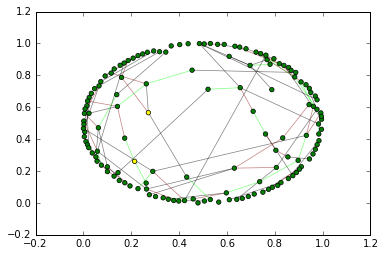
\includegraphics[width=60mm]{grapher01.png}}
     {}
&
\subf{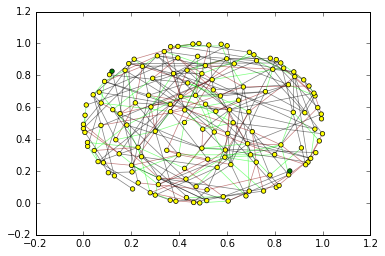
\includegraphics[width=60mm]{grapher03.png}}
     {}
\\
\hline
\subf{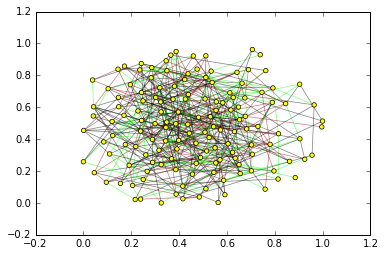
\includegraphics[width=60mm]{grapher05.png}}
     {}
&
\subf{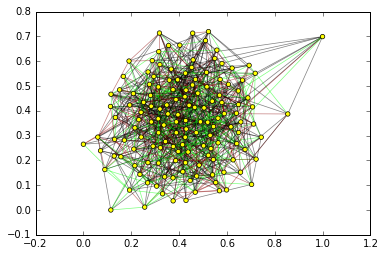
\includegraphics[width=60mm]{grapher09.png}}
     {}
\\
\hline
\end{tabular}
\caption{}
\end{figure}


\begin{figure}[h]
\centering
\begin{tabular}{|c|c|}
\hline
\subf{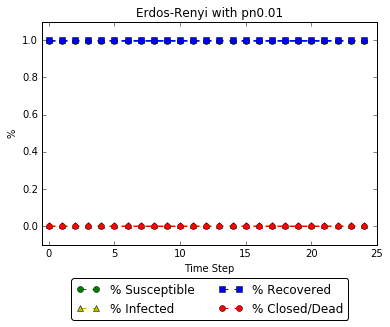
\includegraphics[width=60mm]{ploter01.png}}
     {}
&
\subf{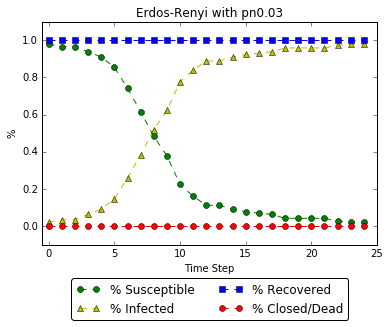
\includegraphics[width=60mm]{ploter03.png}}
     {}
\\
\hline
\subf{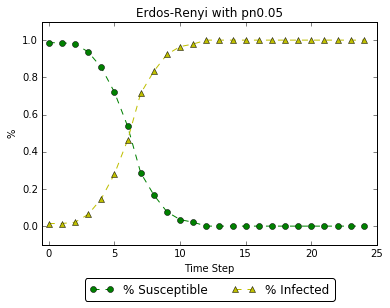
\includegraphics[width=60mm]{ploter05.png}}
     {}
&
\subf{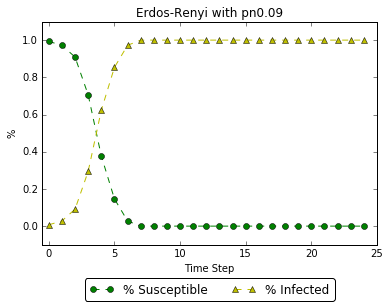
\includegraphics[width=60mm]{ploter09.png}}
     {}
\\
\hline
\end{tabular}
\caption{}
\end{figure}

\subsubsection*{Real Airport Graph and subgraphs}

\subsection*{Simulation 2}
\subsubsection*{Erdos-Renyi Graphs}

\begin{table}[h]
\centering
\caption{My caption}
\label{my-label}
\begin{tabular}{|l|l|l|l|l|l|l|}
\hline
p         & 0.01 & 0.03 & 0.05 & 0.07 & 0.09 & 0.11 \\ \hline
Diameter  & inf  & 8    & 5    & 4    & 3    & 4    \\ \hline
Dead Step & None & None & 17   & None & 11   & 9    \\ \hline
\end{tabular}
\end{table}

\begin{figure}[h]
\centering
\begin{tabular}{|c|c|}
\hline
\subf{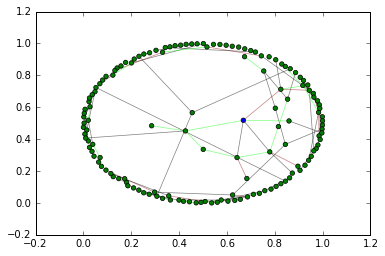
\includegraphics[width=60mm]{graphdie01.png}}
     {}
&
\subf{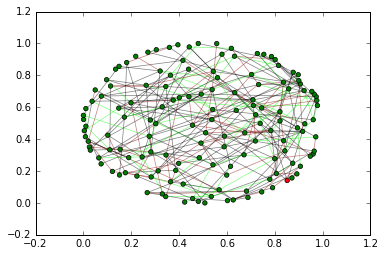
\includegraphics[width=60mm]{graphdie03.png}}
     {}
\\
\hline
\subf{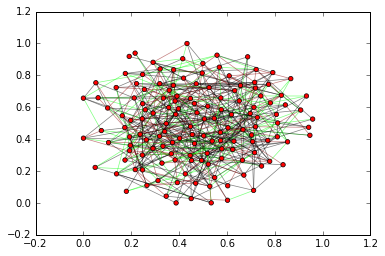
\includegraphics[width=60mm]{graphdie05.png}}
     {}
&
\subf{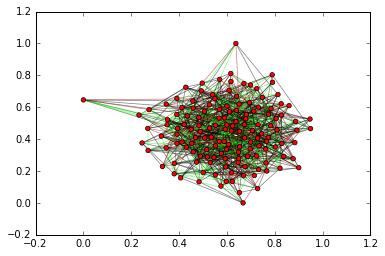
\includegraphics[width=60mm]{graphdie09.png}}
     {}
\\
\hline
\end{tabular}
\caption{}
\end{figure}

\begin{figure}[h]
\centering
\begin{tabular}{|c|c|}
\hline
\subf{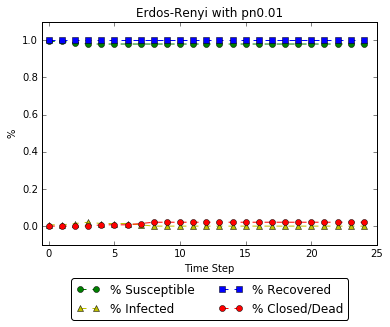
\includegraphics[width=60mm]{ploterdie01.png}}
     {}
&
\subf{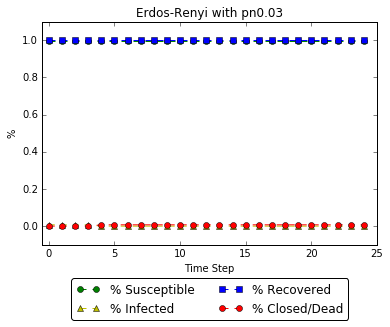
\includegraphics[width=60mm]{ploterdie03.png}}
     {}
\\
\hline
\subf{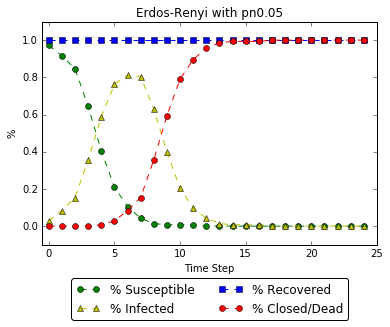
\includegraphics[width=60mm]{ploterdie05.png}}
     {}
&
\subf{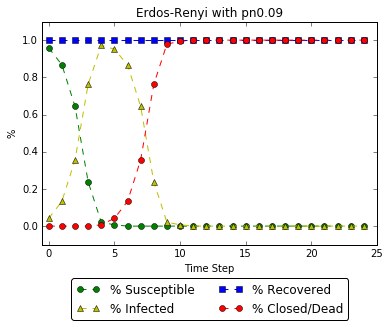
\includegraphics[width=60mm]{ploterdie09.png}}
     {}
\\
\hline
\end{tabular}
\caption{}
\end{figure}

\subsection*{Simulation 3}

\begin{table}[h]
\centering
\caption{My caption}
\label{my-label}
\begin{tabular}{|l|l|l|l|l|l|l|}
\hline
p         & 0.01 & 0.03 & 0.05 & 0.07 & 0.09 & 0.11 \\ \hline
Diameter  & inf  & inf   & 5    & 4    & 4    & 3    \\ \hline
Rec Step & None & None & None   & None & None   & None    \\ \hline
\end{tabular}
\end{table}

\subsubsection*{Erdos-Renyi Graphs}
\begin{figure}[h]
\centering
\begin{tabular}{|c|c|}
\hline
\subf{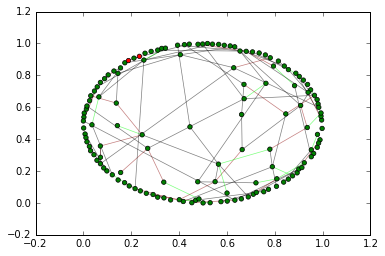
\includegraphics[width=60mm]{graphrec01.png}}
     {}
&
\subf{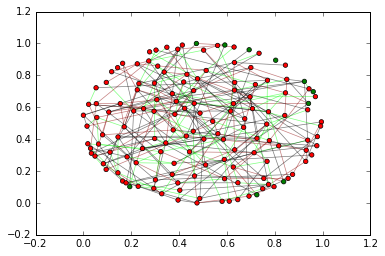
\includegraphics[width=60mm]{graphrec03.png}}
     {}
\\
\hline
\subf{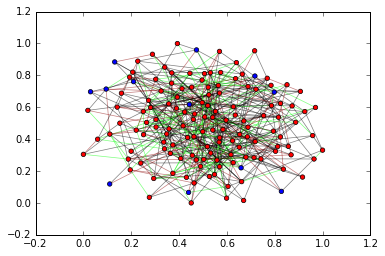
\includegraphics[width=60mm]{graphrec05.png}}
     {}
&
\subf{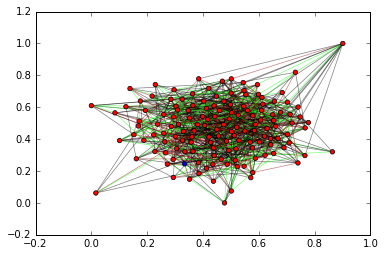
\includegraphics[width=60mm]{graphrec09.png}}
     {}
\\
\hline
\end{tabular}
\caption{}
\end{figure}

\begin{figure}[h]
\centering
\begin{tabular}{|c|c|}
\hline
\subf{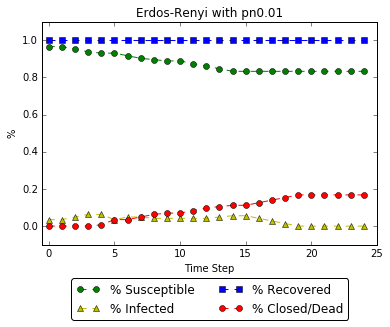
\includegraphics[width=60mm]{plotrec01.png}}
     {}
&
\subf{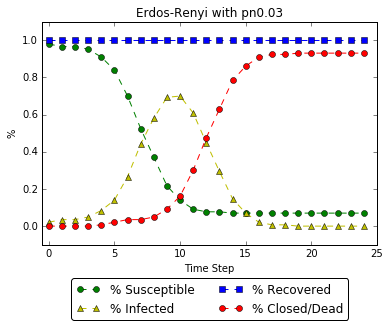
\includegraphics[width=60mm]{plotrec03.png}}
     {}
\\
\hline
\subf{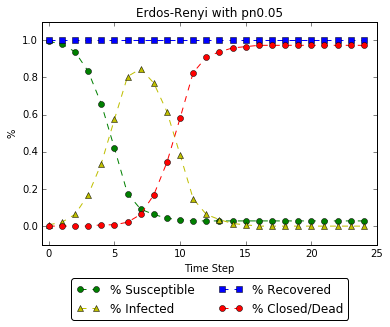
\includegraphics[width=60mm]{plotrec05.png}}
     {}
&
\subf{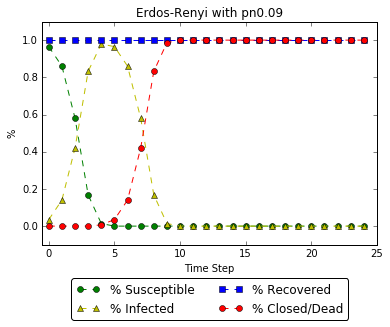
\includegraphics[width=60mm]{plotrec09.png}}
     {}
\\
\hline
\end{tabular}
\caption{}
\end{figure}

\end{document}